\subsection{题目描述}
Search for the minimum of the function \boldmath\( g(x, y) = \sin(x + y) + \cos(x + 2y) \)\unboldmath\ in the whole space.
\subsection{程序描述}
原本这道题是我更感兴趣的,但第一题已经耗费我大量的时间,只能简单实现了四种有名的优化算法:最速下降法,共轭梯度下降法,模拟退火,遗传算法。尤其是共轭梯度下降法,在\textit{Numerical Recipes}的$\S 10.6$中有详细的介绍,不得不承认这书写得还行。以及之前一直没搞懂的命名错误,最速下降法的最速\footnote{\textit{但武思怡前辈分享的最速下降法好像是另一个意思,疑惑\&学习ing。}}原来不代表\textit{Learning Rate} \( \alpha\)是有调节器的,而是指古老的固定步长。而共轭梯度法则是在新的“共轭方向”上进行搜索,这样可以避免最速下降法的\textit{zig zag}现象,当然施法范围有限,主要对二次型和稀疏矩阵有效。模拟退火算法使我想起了大一和伙伴们电磁学荣誉课的\textit{Thompson}问题优化,强大的谢院士当时写的就是这个,龚老师还回信了hhh。遗传算法感觉没有名字那么玄妙,反倒有一种抽奖的感觉,不过可能也因此它的适用范围更广吧。四种算法中前两者是需要梯度的,后面的更普适一些,就像不要导数的Brent求根法。在\textit{Numerical Recipes}的$\S 10.4$还学到了一种不同于它们的\textit{Downhill Simplex Method}方法,它不依赖于分量的一维优化,而是更直接的缩放、反射操作,但没时间实现了...




使用\Colorbox{cmdbg}{\lstinline[language=bash]|g++ *.cpp -o main|}编译,\Colorbox{cmdbg}{\lstinline[language=bash]|./main|}运行(也有已经编译好的\texttt{main.exe}),按照提示可以选择各类方法或者一起比较,也可以自定义各种算法初始值。
\subsection{伪代码}
\begin{algorithm}[H]
    \caption{Steepest Descent Method}
    \label{alg:steepest_descent}
    \KwIn{$x_0$, $y_0$ (float), $\alpha$ (float), \texttt{maxIter} (int), \texttt{tol} (float)}
    \KwOut{$x$, $y$ (float) \tcp*[r]{Approximate minimum}}

    $x \gets x_0$, $y \gets y_0$\;
    \For{$i \gets 1$ \textbf{to} \texttt{maxIter}}{
        \Compute gradient $\nabla f(x, y)$\;
        \If{$\|\nabla f(x, y)\| < \texttt{tol}$}{
            \Break\tcp*[r]{Convergence achieved}
        }
        $(x, y) \gets (x, y) - \alpha \cdot \nabla f(x, y)$\tcp*[r]{Update variables}
    }
    \Return $x$, $y$
\end{algorithm}
\vspace{5pt}
\begin{algorithm}[H]
    \caption{Nonlinear Conjugate Gradient Method (Fletcher-Reeves)}
    \label{alg:conjugate_gradient}
    \KwIn{$x_0$, $y_0$ (float), \texttt{maxIter} (int), \texttt{tol} (float)}
    \KwOut{$x$, $y$ (float) \tcp*[r]{Approximate minimum}}

    $x \gets x_0$, $y \gets y_0$\;
    $\nabla f \gets \nabla f(x, y)$\;
    $\mathbf{d} \gets -\nabla f$ \tcp*[r]{Initial search direction}
    \For{$i \gets 1$ \textbf{to} \texttt{maxIter}}{
        \tcp{Backtracking Line Search (Armijo Condition)}
        \tcp{Find step size $\alpha$ such that}
        \[
            f(x + \alpha d_x, y + \alpha d_y) \leq f(x, y) + c \cdot \alpha \cdot (\nabla f \cdot \mathbf{d})
        \]
        \tcp*[r]{Determine step size $\alpha$}
        $(x, y) \gets (x, y) + \alpha \cdot \mathbf{d}$\;
        $\nabla f_{\text{new}} \gets \nabla f(x, y)$\;
        \If{$\|\nabla f_{\text{new}}\| < \texttt{tol}$}{
            \Break \tcp*[r]{Convergence achieved}
        }
        $\beta \gets \dfrac{\|\nabla f_{\text{new}}\|^2}{\|\nabla f\|^2}$ \tcp*[r]{Fletcher-Reeves coefficient}
        $\mathbf{d} \gets -\nabla f_{\text{new}} + \beta \cdot \mathbf{d}$\;
        $\nabla f \gets \nabla f_{\text{new}}$\;
    }
    \Return $x$, $y$
\end{algorithm}

\vspace{5pt}

\begin{algorithm}[H]
    \caption{Simulated Annealing}
    \label{alg:simulated_annealing}
    \KwIn{$x_0$, $y_0$ (float), $T_0$ (float), \texttt{Tmin} (float), $\alpha$ (float), \texttt{maxIter} (int)}
    \KwOut{$x$, $y$ (float) \tcp*[r]{Approximate minimum}}

    $x \gets x_0$, $y \gets y_0$\;
    $T \gets T_0$ \tcp*[r]{Initial temperature}
    $f_{\text{current}} \gets f(x, y)$ \tcp*[r]{Current function value}
    \For{$i \gets 1$ \textbf{to} \texttt{maxIter} \textbf{and} $T > \texttt{Tmin}$}{
        \tcp{Generate a new candidate solution}
        $x_{\text{new}} \gets x + \mathcal{U}(-0.5, 0.5)$,
        $y_{\text{new}} \gets y + \mathcal{U}(-0.5, 0.5)$\tcp*[r]{ RandomUniform}
        $f_{\text{new}} \gets f(x_{\text{new}}, y_{\text{new}})$\;
        $\Delta \gets f_{\text{new}} - f_{\text{current}}$ \tcp*[r]{Change in function value}

        \tcp{Acceptance Criterion}
        \If{$\Delta < 0$ \textbf{or} $e^{-\Delta / T} > \mathcal{U}(0, 1)$}{
            $x \gets x_{\text{new}}$, $y \gets y_{\text{new}}$ \tcp*[r]{Accept new solution}
            $f_{\text{current}} \gets f_{\text{new}}$ \tcp*[r]{Update current function value}
        }

        $T \gets \alpha \cdot T$ \tcp*[r]{Cool down}
    }
    \Return $x$, $y$
\end{algorithm}



\begin{algorithm}
    \caption{Genetic Algorithm}
    \label{alg:genetic_algorithm}
    \KwIn{Population size \texttt{N}, Generations \texttt{G}, Mutation rate \texttt{pm}, Crossover rate \texttt{pc}}
    \KwOut{Approximate minimum solution $(x, y)$}

    population $\gets \{(x, y) \mid x, y \sim \mathcal{U}(-10, 10)\}$\tcp*[r]{Initialize population randomly}
    evaluate\_fitness(population)\tcp*[r]{Evaluate initial fitness}

    \For{generation $1$ to \texttt{G}}{
        \For{$i \gets 1$ \textbf{to} \texttt{N}}{
            $a, b \gets$ random\_selection(population)\;
            add $\min(a, b)$ to selected\_population\;
        }

        \For{$i \gets 1$ \textbf{to} \texttt{N} step 2}{
            \If{$\mathcal{U}(0,1) < \texttt{pc}$}{
                $\alpha \gets \mathcal{U}(0,1)$\;
                offspring\_1.x $\gets \alpha \cdot$ selected\_population[$i$].x $+$ (1 - $\alpha) \cdot$ selected\_population[$i+1$].x\;
                offspring\_1.y $\gets \alpha \cdot$ selected\_population[$i$].y $+$ (1 - $\alpha) \cdot$ selected\_population[$i+1$].y\;
                offspring\_2.x $\gets \alpha \cdot$ selected\_population[$i+1$].x $+$ (1 - $\alpha) \cdot$ selected\_population[$i$].x\;
                offspring\_2.y $\gets \alpha \cdot$ selected\_population[$i+1$].y $+$ (1 - $\alpha) \cdot$ selected\_population[$i$].y\;
                replace selected\_population[$i$] and [$i+1$] with offspring\_1, offspring\_2\;
            }
        }

        \For{each individual in selected\_population}{
            \If{$\mathcal{U}(0,1) < \texttt{pm}$}{
                individual.x $\gets$ clip(individual.x + $\mathcal{U}(-0.5, 0.5)$, -10, 10)\;
                individual.y $\gets$ clip(individual.y + $\mathcal{U}(-0.5, 0.5)$, -10, 10)\;
            }
            individual.fitness $\gets f(individual.x, individual.y)$\;
        }

        population $\gets$ selected\_population\;
    }

    best $\gets \text{argmin}\{f(x, y) \mid (x, y) \in population\}$\;
    \Return best.x, best.y\;
\end{algorithm}



\subsection{结果示例}
\begin{figure}[H]
    \centering
    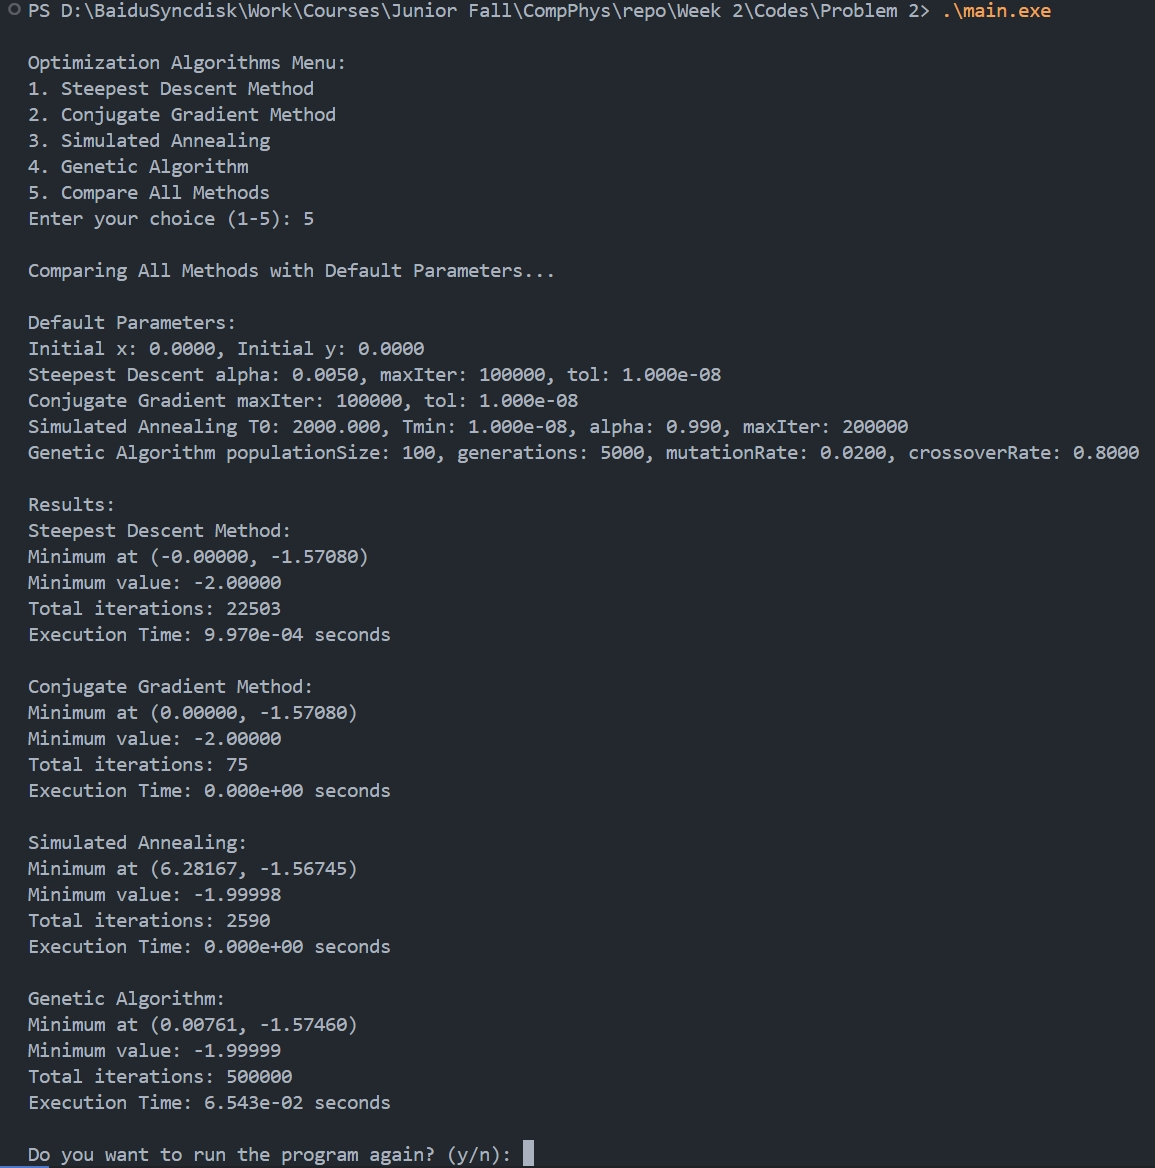
\includegraphics[width=1.0\textwidth]{Figs/2_all.png}
    \caption{\texttt{main.cpp}模式5,对比四种方法}
    \label{fig:2_cpp_all}
\end{figure}
